\section{Introduction}

\begin{frame}
  \note{
    \begin{itemize}
    \item Phases
    \item Definition
    \item Brief overview of the beginning:
      \begin{itemize}
      \item Solvay-like picture
      \item Lot of ideas \& concrete realizations
      \item
      \end{itemize}
    \item Winters
    \end{itemize}
  }
  \frametitle{A brief history of \acs{AI} and \acs{ML}}

  \begin{textblock}{45}(0,15)
    \begin{itemize}
    \item<1-> 1956: birth of \acl{AI}
    \item<3-> 1959: birth of \acl{ML}
    \item<4-> The first years saw the development of many approaches and techniques
    \item<5-> ``Winters'' of \ac{AI}
      \begin{itemize}
      \item Development never halted
      \item Kasparov \vs{} Deep Blue
      \end{itemize}
    \item<6-> Rise of \ac{ML} at the turn of the millennium
    \item<7-> Rise of \acl{DL} since 2012
      \begin{itemize}
      \item AlexNet (2012): first \ac{DL} model to out-performs classical methods
      \end{itemize}
    \end{itemize}
  \end{textblock}

   \begin{textblock}{45}(50,15)
     \only<1>{
       \begin{center}
         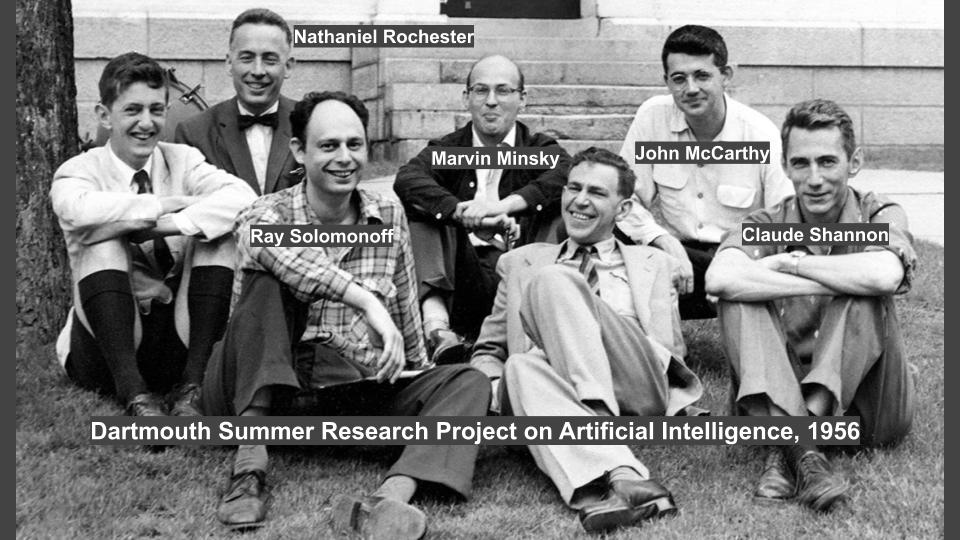
\includegraphics[width=0.9\textwidth]{img/dartmouth-conference.jpg}
       \end{center}
     }
     \only<2>{
       \begin{itemize}
       \item {\footnotesize Discipline focused on creating systems capable of
           performing tasks that typically require human intelligence, such as
           problem-solving, decision-making, translation, \etc{}}
     \end{itemize}
   }
   \only<3>{
     \begin{itemize}
     \item {\footnotesize Field of \ac{AI} focused on the development and study
           of machines that can learn}
     \item {\footnotesize A computer program is said to learn from experience
         E with respect to some class of tasks T and performance measure P if
         its performance at tasks in T, as measured by P, improves with
         experience E (Tom Mitchell).}
     \end{itemize}
   }
   \only<4>{
     \begin{itemize}
     \item Herbert Simon (1958): ``Within ten years a digital computer will be
       the world's chess champion''
     \item John McCarthy: ``As soon as it works, nobody calls it \ac{AI} anymore''
     \end{itemize}
    }
    \only<5>{
      \begin{itemize}
      \item Lighthill report (1973): ``In no part of the field have the
        discoveries made so far produced the major impact that was then
        promised''
      \end{itemize}
    }
    \onslide<6->{
      \begin{itemize}
        \item Practical causes:
          \begin{itemize}
          \item Lots of data
          \item Processing power (GPU) and storage capability
          \item Mature technology (langages, frameworks)
          \end{itemize}
        \item<7-> Neural networks are mature
          \begin{itemize}
          \item Advantage in terms of modularity
          \end{itemize}
        \end{itemize}
    }
   \end{textblock}
 \end{frame}


% Benefits/risks of ML
\begin{frame}
  \note{
    \begin{itemize}
    \item Present benefits and risks
    \item Almost each benefit as a potential counterpart
    \end{itemize}
  }
  \frametitle{Benefits and risks}

  \begin{textblock}{45}(5, 15)
    \begin{block}{Benefits}
      % Large scale deployment of \ac{ML} technology could benefit to:
      \begin{itemize}
      \item Deeper understanding of some phenomena:
        \begin{itemize}
        \item Prediction, classification, \etc{}
        \item Quantitative approach in Social Sciences
        \item Better modelling
        \end{itemize}
      \item Better services:
        \begin{itemize}
        \item Personalized medecine, smart cities, smart grids, \etc{}
        \item Personal assistant
        \end{itemize}
      \end{itemize}
    \end{block}
  \end{textblock}

  \begin{textblock}{45}(50, 15)
    \begin{block}{Risks}<2->
      % Large scale deployment of \ac{ML} technology could be detrimental to:
      \begin{itemize}
      \item Ethical aspects:
        \begin{itemize}
        \item Blind decision, discrimination
        \end{itemize}
      \item Legal aspects:
        \begin{itemize}
        \item Privacy, safety, security, copyrights
        \end{itemize}
      \item Cognitive effects:
        \begin{itemize}
        \item Loss of skills
        \item Attention span
        \end{itemize}
      \item Economical aspects:
        \begin{itemize}
        \item Disparition of jobs
        \item Over-importance of some companies
        \end{itemize}
      \item Environmental impact
      \end{itemize}
    \end{block}
  \end{textblock}
\end{frame}


\subsection{How to go further?}

\begin{frame}
  \note{
    \begin{itemize}
    \item Here are the most important slides
    \end{itemize}
  }
  \frametitle{General books}

  \nocite{*}

  \begin{textblock}{90}(5, 15)
    \begin{block}{AI}<1->
      \printbibliography[heading=none,category=AI]
    \end{block}

    \begin{block}{\ac{ML}}<2->
      \printbibliography[heading=none,category=ML]
    \end{block}
  \end{textblock}
\end{frame}

\begin{frame}
  \frametitle{Deep learning books}

  \nocite{*}

  \begin{textblock}{90}(5, 15)
    \begin{block}{DL}<1->
      \printbibliography[heading=none,category=deep_learning]
    \end{block}
  \end{textblock}
\end{frame}

\begin{frame}
  \frametitle{Courses \& tutorials}

  \begin{textblock}{90}(5, 15)
    \begin{block}{Courses}<1->
      \begin{itemize}
      \item Coursera MOOC:
        \url{https://www.coursera.org/specializations/machine-learning-introduction} (more or less based on \href{https://cs230.stanford.edu/}{Stanford CS230 (Deep Learning)})
      \item FIDLE (Formation Introduction au Deep LEarning): \url{https://fidle.cnrs.fr/}
        (yearly course with practical examples in French)
      \end{itemize}
    \end{block}

    \begin{block}{Challenges}<2->
      \begin{itemize}
      \item Kaggle: \url{https://www.kaggle.com/}
      \item ENS Challenge Data: \url{https://challengedata.ens.fr/}
      \end{itemize}
    \end{block}

    \begin{block}{Tutorials}<3->
      \begin{itemize}
      \item PyTorch tutorials: \url{https://pytorch.org/tutorials/}
      \item scikit-learn tutorials:
        \url{https://scikit-learn.org/stable/user_guide.html}
      \end{itemize}
    \end{block}
  \end{textblock}
\end{frame}
